% !TeX program = pdflatex
\documentclass[tikz,border=8pt]{standalone}
\usepackage{pgfplots}
\usetikzlibrary{arrows.meta}
\pgfplotsset{compat=1.16}
\definecolor{FigureBlue}{HTML}{2563EB}
\definecolor{FigureOrange}{HTML}{EA580C}
\definecolor{FigureSlate}{HTML}{64748B}
\begin{document}
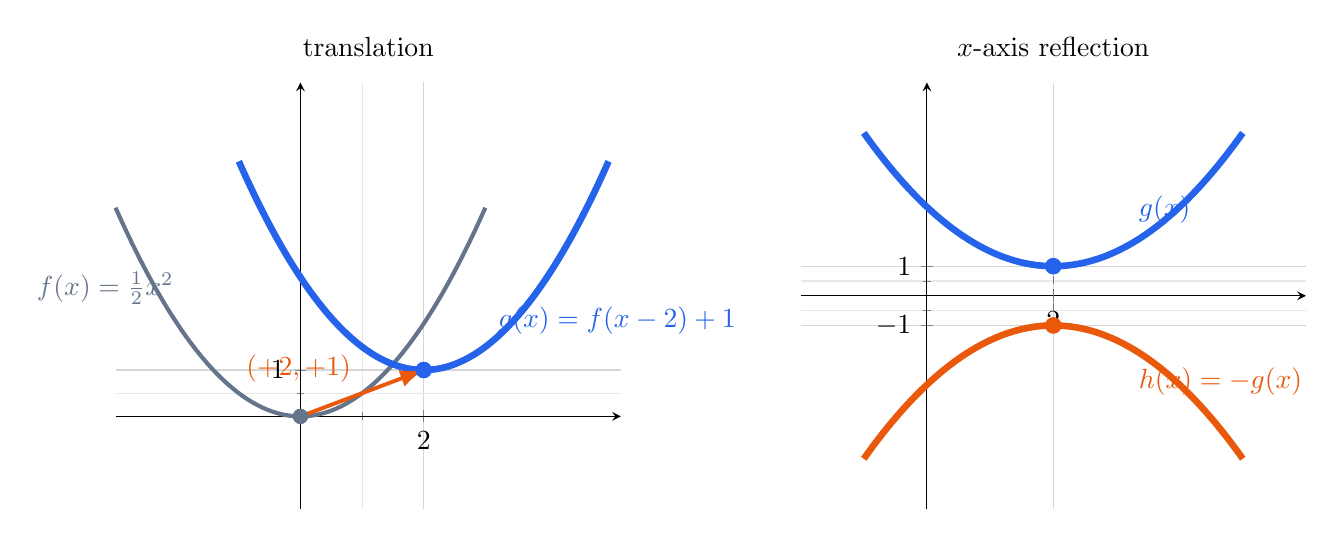
\begin{tikzpicture}
  \begin{axis}[
    name=shift,width=8cm,height=7cm,axis lines=middle,
    xmin=-3,xmax=5.2,ymin=-2,ymax=7.2,xtick={0,2},ytick={0,1},
    title={translation},grid=both,minor tick num=1,clip=false,
    grid style={draw=gray!18},major grid style={draw=gray!32},
  ]
    \addplot[FigureSlate,line width=1.5pt,domain=-3:3,samples=121] {.5*x^2};
    \addplot[FigureBlue,line width=2.4pt,domain=-1:5,samples=121] {.5*(x-2)^2+1};
    \addplot[only marks,mark=*,mark size=2.6pt,FigureSlate] coordinates {(0,0)};
    \addplot[only marks,mark=*,mark size=2.8pt,FigureBlue] coordinates {(2,1)};
    \draw[-{Latex[length=3mm]},FigureOrange,line width=1.4pt]
      (axis cs:0,0)--node[above left] {$(+2,+1)$}(axis cs:2,1);
    \node[anchor=south east,text=FigureSlate] at (axis cs:-1.9,2.2) {$f(x)=\frac12x^2$};
    \node[anchor=south west,text=FigureBlue] at (axis cs:3.05,1.55) {$g(x)=f(x-2)+1$};
  \end{axis}
  \begin{axis}[
    at={(8.7cm,0)},anchor=south west,width=8cm,height=7cm,axis lines=middle,
    xmin=-2,xmax=6,ymin=-7.2,ymax=7.2,xtick={2},ytick={-1,0,1},
    title={$x$-axis reflection},grid=both,minor tick num=1,clip=false,
    grid style={draw=gray!18},major grid style={draw=gray!32},
  ]
    \addplot[FigureBlue,line width=2.4pt,domain=-1:5,samples=121] {.5*(x-2)^2+1};
    \addplot[FigureOrange,line width=2.4pt,domain=-1:5,samples=121] {-(.5*(x-2)^2+1)};
    \addplot[only marks,mark=*,mark size=2.8pt,FigureBlue] coordinates {(2,1)};
    \addplot[only marks,mark=*,mark size=2.8pt,FigureOrange] coordinates {(2,-1)};
    \draw[densely dashed,FigureSlate] (axis cs:2,-1)--(axis cs:2,1);
    \node[anchor=south west,text=FigureBlue] at (axis cs:3.2,2.1) {$g(x)$};
    \node[anchor=north west,text=FigureOrange] at (axis cs:3.2,-2.1) {$h(x)=-g(x)$};
  \end{axis}
\end{tikzpicture}
\end{document}
